\documentclass[tikz]{standalone}
% \standaloneconfig{border=10}
\usepackage{amsthm,amsmath,amsfonts}
\usetikzlibrary{shapes,decorations,arrows,calc,arrows.meta,fit,positioning}
\tikzset{
    -Latex,auto,node distance =2 cm and 2 cm,semithick,
    state/.style ={ellipse, draw, minimum width = 0.7 cm},
    point/.style = {circle, draw, inner sep=0.04cm,fill,node contents={}},
    el/.style = {inner sep=2pt, align=left, sloped}
}
\begin{document}
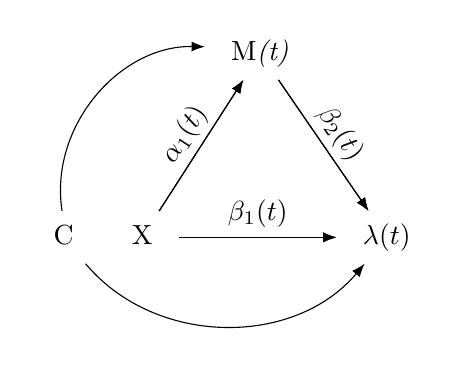
\begin{tikzpicture}
    \node (x) at (-5,0) {\begin{tabular}{c}X\end{tabular}};
    \node (y) [right=of x] {\begin{tabular}{c}$\lambda(t)$\end{tabular}};
    \node (m) [above=of x] at (-3.5,0) {\begin{tabular}{c}M\textit{(t)}\end{tabular}};
    \node[label={[align=center]}] (C) at (-6,0) {\begin{tabular}{c} C \end{tabular}};

    \path (x) edge (y);
    \path (m) edge (y);
    \path (x) edge (m);
    \path (C) edge[bend left=50] (m);
    \path (C) edge[bend right=50] (y);

    \path (x) edge node[above] {$\beta_{1}(t)$} (y);
    \path (x) edge node[el, above] {$\alpha_{1}(t)$} (m);
    \path (m) edge node[el, above] {$\beta_{2}(t)$} (y);
\end{tikzpicture}
\end{document}
